\section{Results}
\label{sec:results}

\subsection{Analysis of the whole road}
\label{sec:results:whole}
In the first part of the analysis a focus has been set on analyzing the road as whole. For each
parameter the road was initialized with still standing cars and was running for about 15 minutes to
reach a state of equilibrium. Although there is a macroscopic equilibrium reached, because of the
variance in desired velocity, there is still a microscopic dynamic.

After the the equilibrium setting in, the maximum average speed gets computed. The result of this
part is shown in \label{fig:speed-cars}. As it can be seen in the plot, there is only a small 
difference between the two models. 

To measure the car throughput, the formula
\[
  \text{Throughput} = \frac{\text{Speed} \cdot \text{\#  of cars}}
  {\text{Lane length} \cdot \text{\# of lanes}}
\]
has been used on the same data set. The resulting plot is shown in \autoref{fig:throughput-cars}.
Since we now have a connection between the speed and throughput, this function has been plotted in
\autoref{fig:throughput-speed}. Since there was only little difference between the two laws in the
first place, there is no further difference to be observed.
\begin{figure}[H]
	\centering
	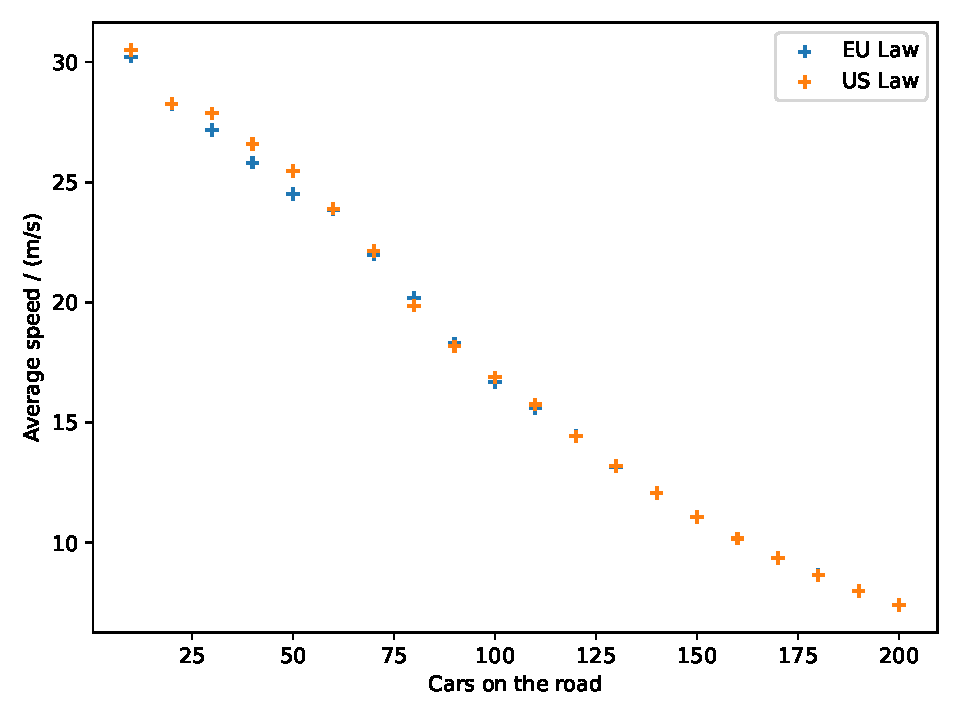
\includegraphics[width=0.9\linewidth]{media/ave_speed_comparison.pdf}
	\caption{Average speed on the road plotted against the amount of cars on the road for US and EU driving law.}
	\label{fig:speed-cars}
\end{figure}

\begin{figure}[H]
	\centering
	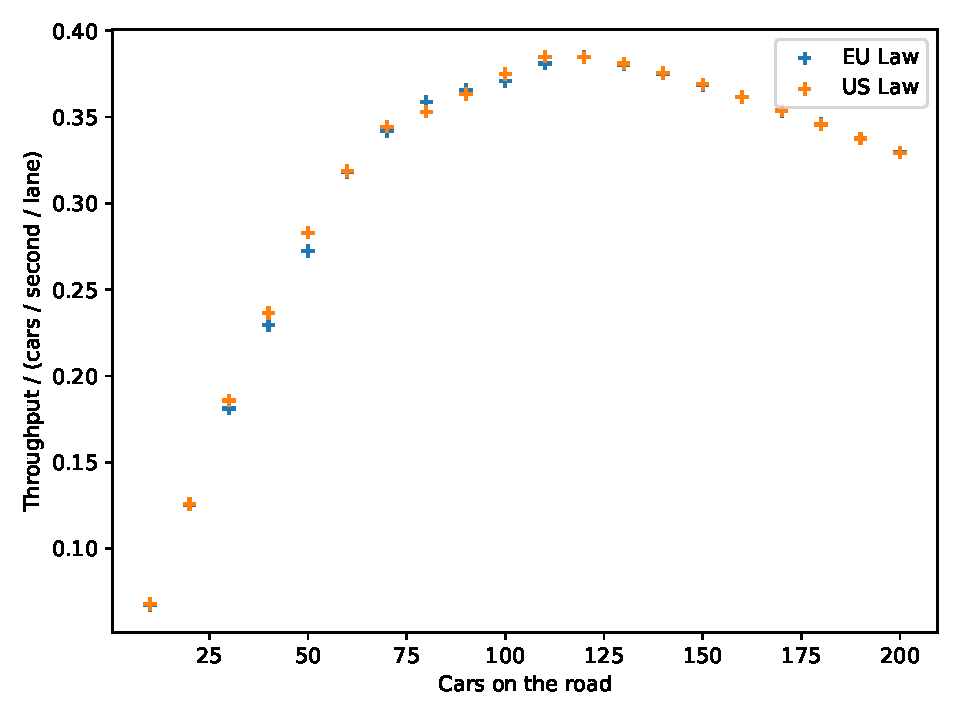
\includegraphics[width=0.9\linewidth]{media/throughput_cars.pdf}
	\caption{Average throughput on the road plotted against the amount of cars on the road for US and EU driving law.}
	\label{fig:throughput-cars}
\end{figure}

\begin{figure}[H]
	\centering
	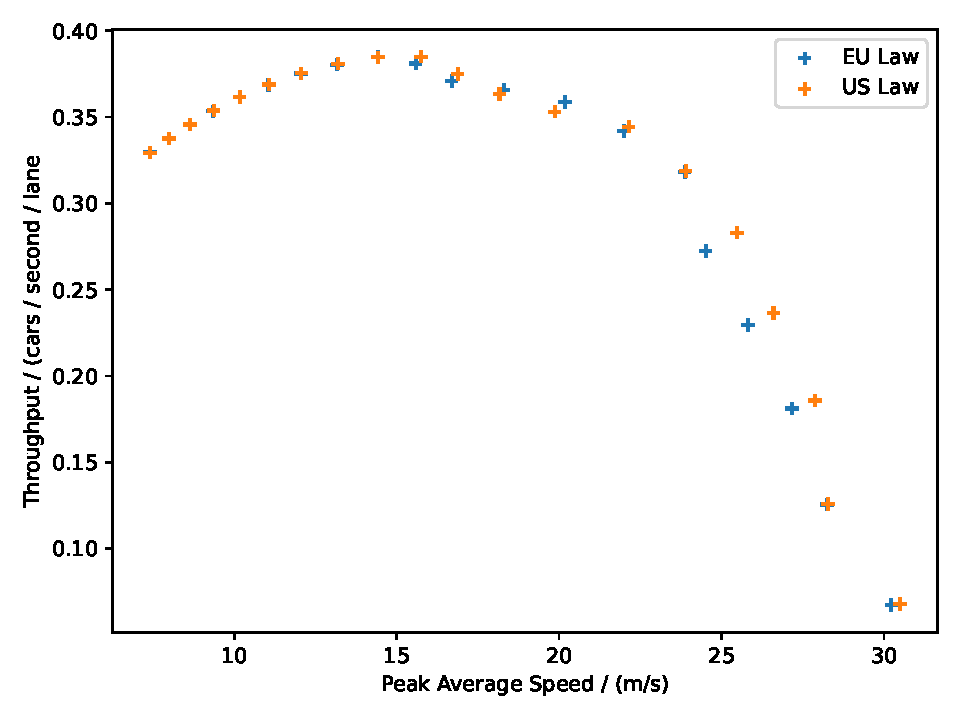
\includegraphics[width=0.9\linewidth]{media/throughput_speed.pdf}
	\caption{Average throughput on the road plotted against the average speed on the road for US and EU driving law.}
	\label{fig:throughput-speed}
\end{figure}
The last plot showed an interesting result about road design: There is no significant difference in
car throughput between $\SI{10}{m/s}$ and $\SI{25}{m/s}$ ($\SI{36}{km/h}$ and $\SI{90}{km/h}$). So
when a car shall achieve maximum car throughput, there is only a small gain from limiting the
traffic to a speed of below $\approx \SI{80}{km/h}$. This result is consitent with real world
studies, comming to conclusion of an optimal speed between $\SI{73}{km/h}$ and $\SI{82}{km/h}$
\cite{HOSSEINLOU201536}.

\subsection{Analysis of individual lanes}
\label{sec:results:indiv}
Since the previous section showed no meaningfull difference when analyzing the whole road, further
work has been done to find a difference on a per-lane basis. As both the simulation and the data
analysis are computationally more expensive here, the amount of cars has been limited to 110. The
higher price comes from a more refined but exact computation, as now about 500 hours of traffic get
simulated. For each run, the average velocity gets computed 20 times with 15 minutes between each
measurement, so that they can be treated as independent measurements.

As it will be seen however, the two models show small variation for such high car densities anyways,
so the benefit of more accurate results outways the loss of data for high car densities.

For readability, the two models have been split up, the per lane analysis is shown in 
\autoref{fig:speed_lanes_EU} and 
\autoref{fig:speed_lanes_US} for the asymmetric and symmetric model respectively.

\begin{figure}[H]
	\centering
	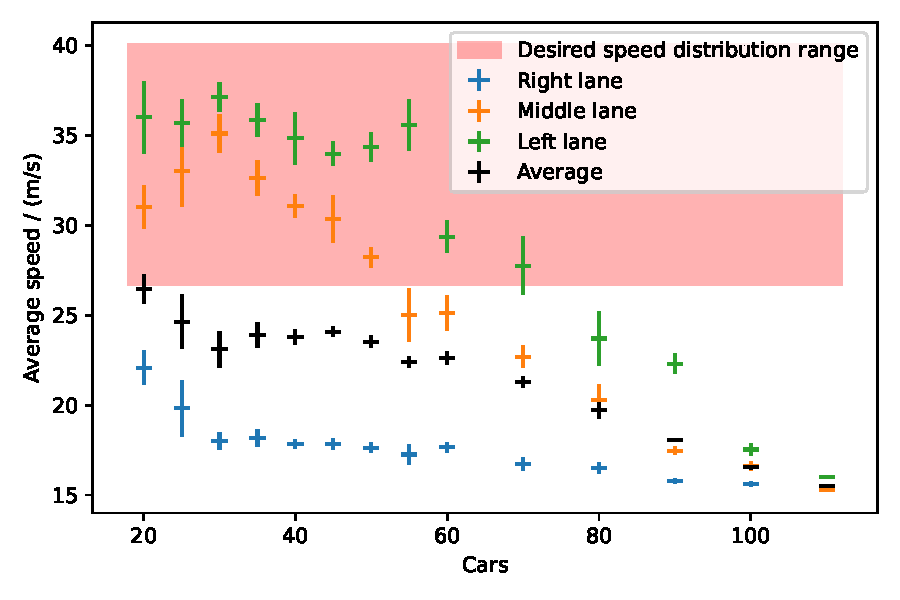
\includegraphics[width=0.9\linewidth]{media/speed_lanes_EU.pdf}
	\caption{Average speed of cars for each lane with the asymmetric driving law.}
	\label{fig:speed_lanes_EU}
\end{figure}
\begin{figure}[H]
	\centering
	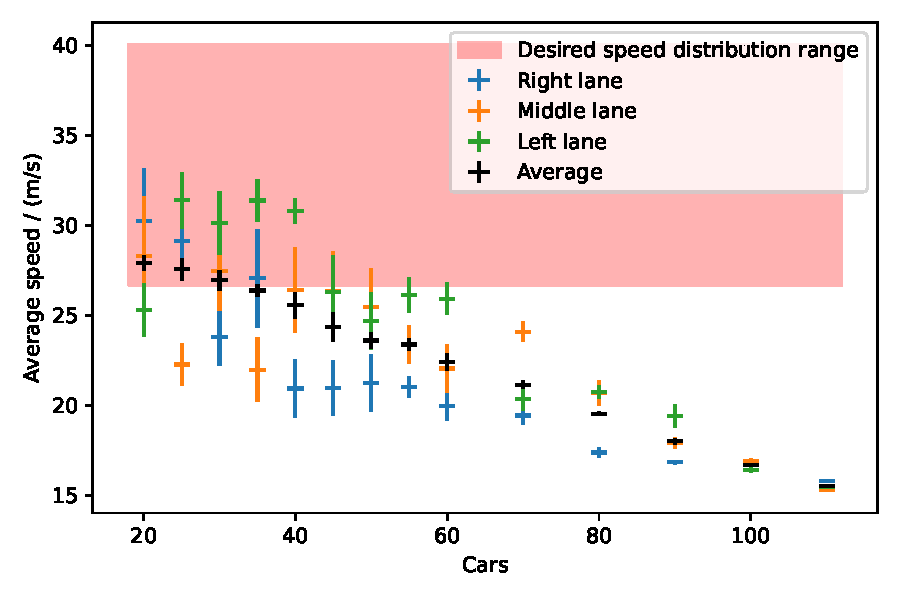
\includegraphics[width=0.9\linewidth]{media/speed_lanes_US.pdf}
	\caption{Average speed of cars for each lane with the symmetric driving law.}
	\label{fig:speed_lanes_US}
\end{figure}
A notable difference here is the small difference between each lane for the US model. This lies in
the nature of the model, but it also means that all lanes get slowed down when more cars are on the
road. When a asymmetric rule is used, the left and middle lanes (so the passing, high speed lanes)
only get a small performance hit until about 60 cars are on the road. 
